\chapter{الجاذبية}\label{ch:g9:gravitation}

تفاحة تفلت من غصنها فتسقط. \omterm{def:g2:moon-in-the-sky:moon}{والقمر}، فوق البستان نفسه، لا يسقط.
وظلّت هاتان حقيقتين لا صلة بينهما آلاف السنين --- حتى جمعتهما
لمحة عبقرية واحدة: \omterm{def:g2:moon-in-the-sky:moon}{فالقمر} \emph{يسقط} بلا انتهاء حول الأرض،
ممسوكًا بالجذب عينه الذي يطالب بالتفاحة. قانون واحد للبستان
والسماء --- أجرأ معادلة كُتبت إلى ذلك اليوم، وبها تفتتح سنتك
الأخيرة في هذا الكتاب.

\section{التجاذب الكوني}

\begin{definition}[الجاذبية]\label{def:g9:gravitation:gravitation}
\emph{الجاذبية}\index{جاذبية} هي التجاذب المتبادل بين الكتل
كلها: فكل قطعة مادة في الكون تجذب كل قطعة أخرى. وهي \omterm{def:g2:pushes-and-pulls:force}{القوة} بلا
لمس التي لقيتها ``جذب الأرض'' منذ سنوات --- وقد تكشّفت الآن
كونيةً: فالأرض تجذب التفاحة، والتفاحة تجذب الأرض، \omterm{def:g2:moon-in-the-sky:moon}{والقمر} يجذب
البحار، والشمس تجذب الكواكب، وكتابان على رفّ يتجاذبان، جذبًا
واهنًا، إلى الأبد.
\end{definition}

\begin{proposition}[قانون الجذب العام]\label{prop:g9:gravitation:law}
جسمان كتلتاهما $m_A$ و$m_B$ (\omterm{def:g6:measurement-in-science:measuring}{بوحدة} \unit{kg})، ومركزاهما على
مسافة $d$ (\omterm{def:g6:measurement-in-science:measuring}{بوحدة} \unit{m})، يتجاذبان بقوّتين متساويتين
متعاكستين على امتداد الخطّ الواصل بينهما، مقدارهما
\[
F = G \times \frac{m_A \times m_B}{d^2},
\]
و$F$ بالنيوتن (\unit{N}) --- \omterm{def:g6:measurement-in-science:measuring}{وحدة} \omterm{def:g2:pushes-and-pulls:force}{القوة} التي تبدأ حكايتها
الكاملة في الفصل التالي --- مع
$G = \qty{6.67e-11}{N.m^2/kg^2}$، وهو \emph{ثابت الجذب}،
العدد نفسه في كل مكان من الكون. \omterm{def:g2:pushes-and-pulls:force}{والقوة} تكبر مع كل \omterm{def:g3:measuring-mass:mass}{كتلة}، وتموت
مع \emph{مربّع} المسافة: فبضعف البعد تضعف أربع مرات، وبعشرة
أضعافه تضعف مئة مرة.
\end{proposition}

\begin{omfigure}
\begin{tikzpicture}[scale=0.85]
  \draw[thick, fill=omDef, fill opacity=0.4] (1.4,1.4) circle (0.65);
  \node[font=\small] at (1.4,1.4) {$m_A$};
  \draw[thick, fill=omThm, fill opacity=0.4] (8.6,1.4) circle (0.45);
  \node[font=\small] at (8.6,1.4) {$m_B$};
  \draw[-Stealth, very thick, omThm] (2.15,1.4) -- (3.55,1.4);
  \draw[-Stealth, very thick, omDef] (8.05,1.4) -- (6.65,1.4);
  \draw[Stealth-Stealth, omExo] (1.4,0.45) -- (8.6,0.45);
  \node[below, font=\small, omExo] at (5.0,0.35) {$d$};
  \node[above, font=\small] at (5.0,1.75)
    {جذبان متساويان في جهتين متعاكستين --- وكلاهما دائمًا};
\end{tikzpicture}

{\small الجذب العام: كتلتان، وجذبان متساويان متعاكسان على
امتداد الخطّ الواصل --- فالتفاحة تجذب الأرض \omterm{def:g2:pushes-and-pulls:force}{بالقوة} نفسها التي
تجذب بها الأرضُ التفاحة.}
\end{omfigure}

\begin{example}[قراءة القانون]\label{ex:g9:gravitation:reading}
كل ملمح في الصيغة يتكلّم. فالكتلتان تتضاربان: ضاعف أيّ شريك
تتضاعف \omterm{def:g2:pushes-and-pulls:force}{القوة}. والمسافة مربّعة في المقام: \omterm{def:g9:gravitation:gravitation}{فالجاذبية} همسة تخبو
سريعًا --- وهو التخفيف بمربّع المسافة الذي ستلقاه ثانية مع
\omterm{def:g1:light-and-shadows:source}{الضوء} \omterm{def:g3:sound-around-us:sound}{والصوت}، إذ هو هندسة كل ما ينتشر في الفضاء. وأمّا صغر $G$
البالغ --- أحد عشر صفرًا بعد الفاصلة --- فيعلن أن \omterm{def:g9:gravitation:gravitation}{الجاذبية} ضعيفة
قوى الطبيعة: ولا تحكم الكون إلا لأن الكتل هناك وحشية ولأن لا
شيء يلغيها.
\end{example}

\begin{example}[لماذا لا ترتطم الرفوف بعضها ببعض]\label{ex:g9:gravitation:books}
كتابان \omterm{def:g3:measuring-mass:mass}{كتلة} كل منهما \qty{1}{kg}، ومركزاهما على \qty{0.1}{m}:
\[
F = \num{6.67e-11} \times \frac{1 \times 1}{0.1^2}
= \qty{6.67e-9}{N}
\]
--- أي أجزاء من مليار من النيوتن، وهي \omterm{def:g4:weight-and-mass:weight}{وزن} ذرّة غبار من ذرّة
غبار. والآن الأرض والتفاحة: استبدل بأحد الكتابين
\qty{5.97e24}{kg} من \omterm{def:g4:solar-system:planet}{الكوكب}، وبالمسافة نصف قطره
\qty{6.4e6}{m}، يسلّم القانون نفسه الشدّ المألوف في أصيل
بستان. فالكوني يعني الكوني --- ولا تقرّر إلا الكتل من يلحظ.
\end{example}

\section{القمر الساقط}

\begin{example}[المدفع على الجبل]\label{ex:g9:gravitation:cannon}
تجربة اللمحة الفكرية نفسها. أطلق قذيفة مدفع أفقيًّا من قمّة
عالية: فترسم قوسًا وتحطّ. أطلقها أسرع: فتحطّ أبعد --- وجذب
الأرض يحني مسارها طول الوقت. والآن تخيّل إطلاقها من \omterm{def:g7:motion-average-speed:formula}{السرعة}
بحيث \emph{ينحني سطح الأرض المستدير هابطًا تحتها بالمعدّل
نفسه} الذي تسقط به: فتسقط القذيفة بلا انتهاء ولا تحطّ أبدًا
--- بل تدور حول \omterm{def:g4:solar-system:planet}{الكوكب}. ولهذا السقوط الدائم اسم مألوف:
\emph{\omterm{def:g6:sun-earth-moon:axisorbit}{مدار}}. فلا شيء يمسك جسمًا مداريًّا ``فوق''؛ بل هو ساقط
بأناقة.
\end{example}

\begin{omfigure}
\begin{tikzpicture}[scale=0.85]
  % the curving Earth: only the upper limb of a much larger circle
  \fill[omDef, opacity=0.25] (-1.01,0.23) arc (106:74:20)
    -- (10.01,-0.9) -- (-1.01,-0.9) -- cycle;
  \draw[thick] (-1.01,0.23) arc (106:74:20);
  % the mountain and its gun
  \draw[thick, fill=omExo!30]
    (-1.1,0.2) -- (0.25,2.3) -- (1.3,0.72) -- cycle;
  \draw[thick, fill=omExo!60] (0.0,2.18) rectangle (0.55,2.42);
  \node[left, font=\small] at (-0.85,2.3) {مدفع الجبل};
  % three shots, each faster than the last
  \draw[omThm, thick] (0.55,2.32)
    .. controls (1.6,2.25) .. (2.4,0.9);
  \draw[omThm, thick] (0.55,2.35)
    .. controls (2.8,2.25) .. (4.9,1.0);
  \draw[omThm, thick] (0.55,2.38)
    .. controls (4.2,2.35) .. (7.5,0.8);
  \node[right, font=\small, omThm] at (1.9,3.0)
    {أسرع: أبعد};
  % fast enough: the fall closes into an orbit
  \draw[omMeth, very thick, dashed] (0.3,2.35) arc (101:73:21.76);
  \node[right, font=\small, omMeth] at (6.4,3.35)
    {بسرعة كافية: يصير السقوط مدارًا};
\end{tikzpicture}

{\small مدفع الجبل: كل طلقة أسرع تسقط أبعد حول الأرض المنحنية
--- حتى يتطابق السقوط والانحناء، فتدور القذيفة في \omterm{def:g6:sun-earth-moon:axisorbit}{مدار}.}
\end{omfigure}

\begin{proposition}[ما تديره الجاذبية]\label{prop:g9:gravitation:runs}
قانون واحد، والسماء كلها: \omterm{def:g2:moon-in-the-sky:moon}{فالقمر} قذيفة مدفع الأرض الأبدية،
يسقط حولنا مرة في الشهر؛ والكواكب تسقط كذلك حول الشمس ---
أقربها أسرع، كما يقتضي مربّع المسافة؛ والمذنّبات تنقضّ من
الظلام في حلقات سقوط طويلة؛ وكل \omterm{def:g2:moon-in-the-sky:moon}{قمر} صناعي --- عيون الطقس،
ومنارات الملاحة، والمحطّة المأهولة الدائرة كل تسعين دقيقة ---
يركب رياضيات مدفع الجبل. فلا شيء في السماوات معلَّق. بل كل شيء
يسقط، ويخطئ الهدف.
\end{proposition}

\begin{example}[المدّ والجزر: القمر يجذب بدوره]\label{ex:g9:gravitation:tides}
للتبادل توقيع مكتوب في الماء. فجذب \omterm{def:g2:moon-in-the-sky:moon}{القمر} للأرض أقوى ما يكون
على المحيط المواجه له وأضعف ما يكون على الجانب البعيد ---
فتتكوّم البحار برفق نحو \omterm{def:g2:moon-in-the-sky:moon}{القمر} وبعيدًا عنه في آن واحد، وبينما
تدور الأرض تحت الكومتين ترى السواحل الماء يعلو ويهبط:
\emph{المدّ والجزر}، مرتين في معظم الأيام. وتضيف الشمس يدها ---
باصطفافها عند المحاق \omterm{ex:g2:moon-in-the-sky:shapes}{والبدر} في مدّ الربيع العظيم. وقد قرأ
الصيّادون \omterm{def:g2:moon-in-the-sky:moon}{القمر} آلاف السنين؛ والقانون يقرؤه لهم.
\end{example}

\begin{remark}[ما لا يقوله القانون]\label{rem:g9:gravitation:notsay}
المعادلة العظيمة تحسب \omterm{def:g2:pushes-and-pulls:force}{القوة} بدقّة رائعة ولا تشرح ذرّة من
\emph{كيف} يمسك جسمان أحدهما بالآخر عبر العدم الفارغ --- وقد
سمّى صاحبها نفسه السؤال مفتوحًا وتركه، بجلال، بلا جواب. وثمّة
أجوبة أعمق --- وسنوات الجامعة في هذا المنهج تبلغ الجواب الحديث،
حيث تحني \omterm{def:g3:measuring-mass:mass}{الكتلة} هندسة المكان الذي تسكنه --- لكن كل فيزيائي أمين
منذ ذلك الحين كرّر الدرس الذي يجوز لك أن تأخذه من هذه الصفحة:
قد يكون القانون نافعًا تمامًا، مختبَرًا تمامًا، وهو مع ذلك
يحرس سرّه الأخير.
\end{remark}

\begin{omfigure}
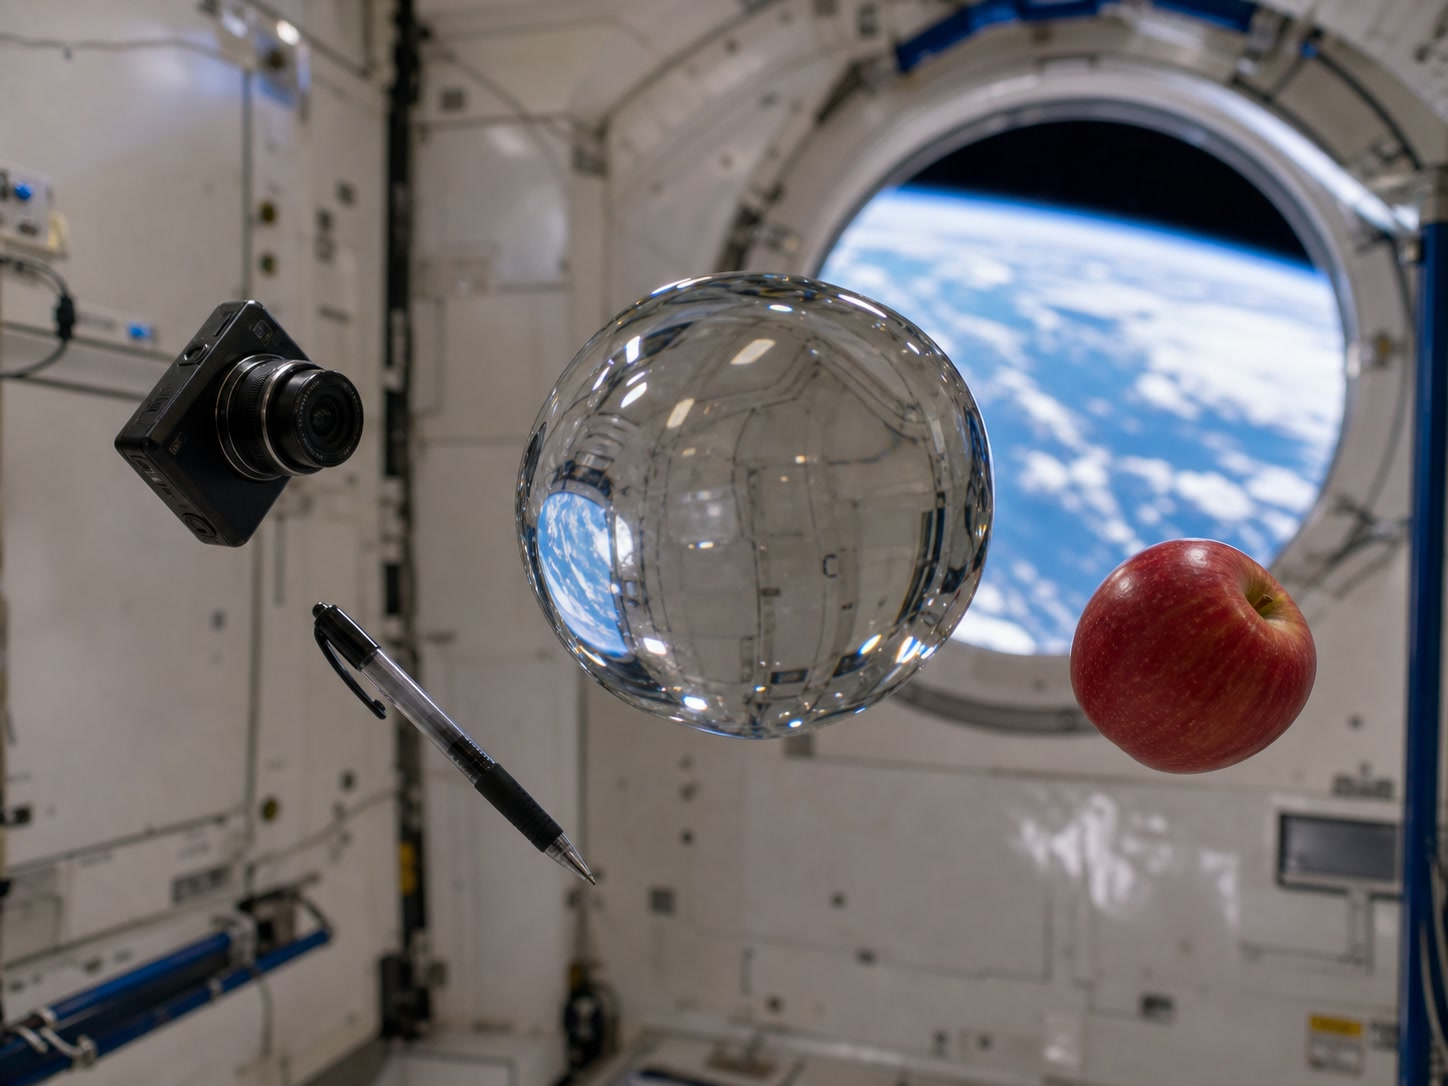
\includegraphics[width=0.5\linewidth]{images/book1/ai/g9-gravitation-weightless.jpg}

{\small السقوط الحرّ معيشًا كل يوم: المحطّة الفضائية وكل ما فيها تسقط حول الأرض معًا، فلا يضغط شيء على شيء --- فتطفو آلات التصوير والأقلام والتفاح والماء.}
\end{omfigure}

\section{تمارين}

\begin{exercise}[$\star$]\label{exo:g9:gravitation:1}
اذكر قانون الجذب العام --- الصيغة والوحدات، والملمحين
(الكتلتان والمسافة) بالكلام.
\end{exercise}

\begin{exercise}[$\star$]\label{exo:g9:gravitation:2}
تجذب الأرض التفاحة \omterm{def:g2:pushes-and-pulls:force}{بقوة} \qty{1}{N}. فبأيّ \omterm{def:g2:pushes-and-pulls:force}{قوة} تجذب التفاحة
الأرضَ؟ ولماذا لا يتسارع بصورة مرئية إلا واحد منهما؟
\end{exercise}

\begin{exercise}[$\star$]\label{exo:g9:gravitation:3}
قمران صناعيان يدوران على مسافتَي $d$ و$2d$ من مركز الأرض.
قارن قوّتَي \omterm{def:g9:gravitation:gravitation}{الجاذبية} عليهما (بكتلتين متساويتين). وعند $10 d$؟
\end{exercise}

\begin{exercise}[$\star$]\label{exo:g9:gravitation:4}
احسب التجاذب بين شريكَي رقص \omterm{def:g3:measuring-mass:mass}{كتلة} كلٍّ منهما \qty{80}{kg} على
بعد \qty{0.5}{m} --- وعلّق على الرومانسية في مقابل \omterm{def:g9:gravitation:gravitation}{الجاذبية}.
\end{exercise}

\begin{exercise}[$\star$]\label{exo:g9:gravitation:5}
في حكاية مدفع الجبل، أيّ معدّلين يتطابقان تمامًا للطلقة
المدارية؟ وما \omterm{def:g6:sun-earth-moon:axisorbit}{المدار}، في ثلاث كلمات؟
\end{exercise}

\begin{exercise}[$\star$]\label{exo:g9:gravitation:6}
``\omterm{def:g1:floating-and-sinking:words}{يطفو} روّاد الفضاء لأنه لا \omterm{def:g9:gravitation:gravitation}{جاذبية} هناك في الأعلى.'' اهدم هذا
بقذيفة المدفع: ماذا تفعل المحطّة وطاقمها كلاهما؟
\end{exercise}

\begin{exercise}[$\star$]\label{exo:g9:gravitation:7}
لماذا تحكم \omterm{def:g9:gravitation:gravitation}{الجاذبية}، ضعيفة الطبيعة، الكونَ مع ذلك؟ سببان من
الفصل.
\end{exercise}

\begin{exercise}[$\star$]\label{exo:g9:gravitation:8}
من أين يجيء المدّ والجزر، ولماذا مرتين في معظم الأيام؟ ومتى
يضرب أعظمها؟
\end{exercise}

\begin{exercise}[$\star\star$]\label{exo:g9:gravitation:9}
\omterm{def:g2:moon-in-the-sky:moon}{القمر} (\qty{7.3e22}{kg}) يدور على \qty{3.8e8}{m} من الأرض
(\qty{5.97e24}{kg}). احسب تجاذبهما، بالكتابة العلمية من أول
السطر إلى آخره --- وتأمّل كم رقمًا تحمل قوة العشرة في
الجواب.
\end{exercise}

\begin{exercise}[$\star\star$]\label{exo:g9:gravitation:10}
على سطح \omterm{def:g2:moon-in-the-sky:moon}{القمر} تقلّص وزنك إلى السدس (تذكّر روّاد الفضاء
النطّاطين). باستعمال قرصَي القانون --- \omterm{def:g3:measuring-mass:mass}{كتلة} \omterm{def:g2:moon-in-the-sky:moon}{القمر} الأصغر،
ونصف قطره الأصغر --- اشرح كيف يظهر سدس من جرم أخفّ من الأرض
ثمانين مرة.
\end{exercise}

\begin{exercise}[$\star\star$]\label{exo:g9:gravitation:11}
عطارد يلفّ حول الشمس في $88$ يومًا، ونبتون في $165$ سنة.
استخرج هذا النمط من مربّع المسافة: ماذا يفعل خبوّ \omterm{def:g9:gravitation:gravitation}{الجاذبية} مع
البعد بقبضة الشمس، ومن ثمّ بوتيرة العائلة الخارجية؟
\end{exercise}

\begin{exercise}[$\star\star\star$]\label{exo:g9:gravitation:12}
\omterm{def:g2:moon-in-the-sky:moon}{قمر} صناعي مستقرّ فوق نقطة واحدة من خطّ الاستواء يبدو ساكنًا
--- فأطباق الهوائيات لا تتحرّك أبدًا. وفّق بين المظهر
و\cref{prop:g9:gravitation:runs}: كم يجب أن يكون دوره
المداري، وفي أيّ جهة يجب أن يدور، ولماذا يعني ``التعلّق'' هنا
``السقوط على خطوة تامّة مع الأرض الدائرة''؟
\end{exercise}

\section{مسألة: ميراث قذيفة المدفع}

\begin{problem}[{مسألة نهاية الأسبوع --- من البستان إلى
المدار؛ التفاحة والمدفع والقمر مدقَّقة بقانون واحد؛ لوحة
إطلاق الأقمار الصناعية}]\label{pb:g9:gravitation:1}
أمسية عند مكتب التوعية في وكالة الفضاء: قانون واحد،
و$G = \qty{6.67e-11}{N.m^2/kg^2}$، \omterm{def:g3:measuring-mass:mass}{وكتلة} الأرض
\qty{5.97e24}{kg}، ونصف قطر الأرض \qty{6.4e6}{m}.

\medskip\noindent\textbf{القسم الأول --- تدقيق التفاحة.}
\begin{enumerate}
  \item احسب جذب الأرض لتفاحة كتلتها \qty{0.1}{kg} عند السطح
        (والمركزان يفصل بينهما نصف قطر أرضي واحد).
  \item وبأيّ \omterm{def:g2:pushes-and-pulls:force}{قوة} تجذب التفاحة الأرض بدورها؟ اذكر كلمة
        القانون لهذه المحاسبة ذات الاتجاهين.
  \item ارفع التفاحة إلى ضعف نصف قطر الأرض من المركز. فماذا
        يصير الجذب؟
  \item ويسأل زائر لماذا تستعمل الصيغة المسافة إلى
        \emph{مركز} الأرض لا إلى الأرض تحت قدميه. قدّم
        الجواب القصير الأمين (\omterm{def:g4:solar-system:planet}{فالكوكب} كله يجذب، وجذوبه
        المتفرّقة تجتمع كأنها من المركز --- وهي مبرهنة
        احتاج صاحب القانون العظيم نفسه سنوات ليثبتها).
\end{enumerate}

\medskip\noindent\textbf{القسم الثاني --- لوحة الإطلاق.}
\begin{enumerate}[resume]
  \item \omterm{def:g3:measuring-mass:mass}{كتلة} \omterm{def:g2:moon-in-the-sky:moon}{قمر} اليوم الصناعي \qty{2000}{kg}. فما وزنه عند
        السطح، بالقانون؟ (أو بالاختصار الذي يسمّيه الفصل
        التالي: نحو \qty{9.8}{N} لكل \omterm{def:g3:measuring-mass:units}{كيلوغرام}.)
  \item وفي مداره العامل على \qty{1.28e7}{m} من المركز ---
        أي نصفَي قطر أرضيين --- أيّ جزء من وزنه السطحي ما
        زالت \omterm{def:g9:gravitation:gravitation}{الجاذبية} تمارسه عليه؟
  \item ``إذن ما زالت هناك \omterm{def:g9:gravitation:gravitation}{جاذبية} حقيقية في الأعلى؟'' أكّد
        بالعدد --- واشرح ماذا يفعل \omterm{def:g2:moon-in-the-sky:moon}{القمر} الصناعي بذلك الجذب
        بدل أن يرتطم.
  \item ويقول تعليق الإطلاق: ``يجب أن تطابق \omterm{def:g7:motion-average-speed:formula}{السرعة} المدارية
        السقوط''. أعِد سرد حكاية مدفع الجبل في جملتين لنشرة
        الزوّار.
\end{enumerate}

\medskip\noindent\textbf{القسم الثالث --- دفتر \omterm{def:g2:moon-in-the-sky:moon}{القمر}.}
\begin{enumerate}[resume]
  \item \omterm{def:g2:moon-in-the-sky:moon}{والقمر} على \qty{3.8e8}{m}، فكم نصف قطر أرضي يركب
        بعيدًا؟ (برقم عشري واحد.)
  \item وبمربّع المسافة، إلى أيّ جزء تقريبًا خبت \omterm{def:g9:gravitation:gravitation}{الجاذبية}
        هناك عن قوّتها السطحية؟ (ربّع جوابك السابق.)
  \item واللمحة العظيمة، معادًا سردها: تفاحة البستان تسقط نحو
        خمسة أمتار في ثانيتها الأولى؛ \omterm{def:g2:moon-in-the-sky:moon}{والقمر}، في كل ثانية،
        ``يسقط'' نحو الأرض بالكاد ملّيمترًا --- ومع ذلك لا
        يصل أبدًا. اربط الحقيقتين عبر جوابَي السؤالين 9 و10:
        لماذا يكون سقوط \omterm{def:g2:moon-in-the-sky:moon}{القمر} أرفق آلاف المرات، ولماذا يكون
        بلا انتهاء؟
  \item اختم أمسية التوعية: قانون واحد، وثلاثة مؤدّين ---
        تفاحة، \omterm{def:g2:moon-in-the-sky:moon}{وقمر} صناعي، \omterm{def:g2:moon-in-the-sky:moon}{وقمر}. اكتب جملة اللوحة الختامية
        التي توحّدهم.
\end{enumerate}
\end{problem}
